\section{friendship}





\subsection{access modifiers}

\begin{frame}[fragile]{access modifiers}
	Wir kennen bereits für die member von Klassen (\verb|class|, \verb|struct|, \verb|union|).
	Wenn man sagt, eine Klasse habe Zugriff auf einen member, so bedeutet dies, dass die member dieser Klasse diesen Zugriff besitzten (z.B. member functions).
	
	\pause
	\hspace{1em}
	
	\begin{block}{Zugriffskontrolle für member}
		Zugriff für member in einer Klasse A für:
		\begin{itemize}
			\item \verb|public| -- jeden
			\item \verb|protected| -- nur die Klasse A selbst und deren Kindklassen
			\item \verb|private| -- nur die Klasse A selbst
		\end{itemize}
	\end{block}
\end{frame}


\begin{frame}{encapsulation \& information hiding}
	\begin{itemize}
		\item Faustregel: Alles so weit wie möglich schützen!
		\item data member i.d.R. private
		\item nur sichere, in sich geschlossene Funktionen public
	\end{itemize}
\end{frame}


\begin{frame}{friendship}
	Friendship erlaubt eine feinere Kontrolle über member access:
	
	\vspace{1em}
	
	\onslide*<+> { 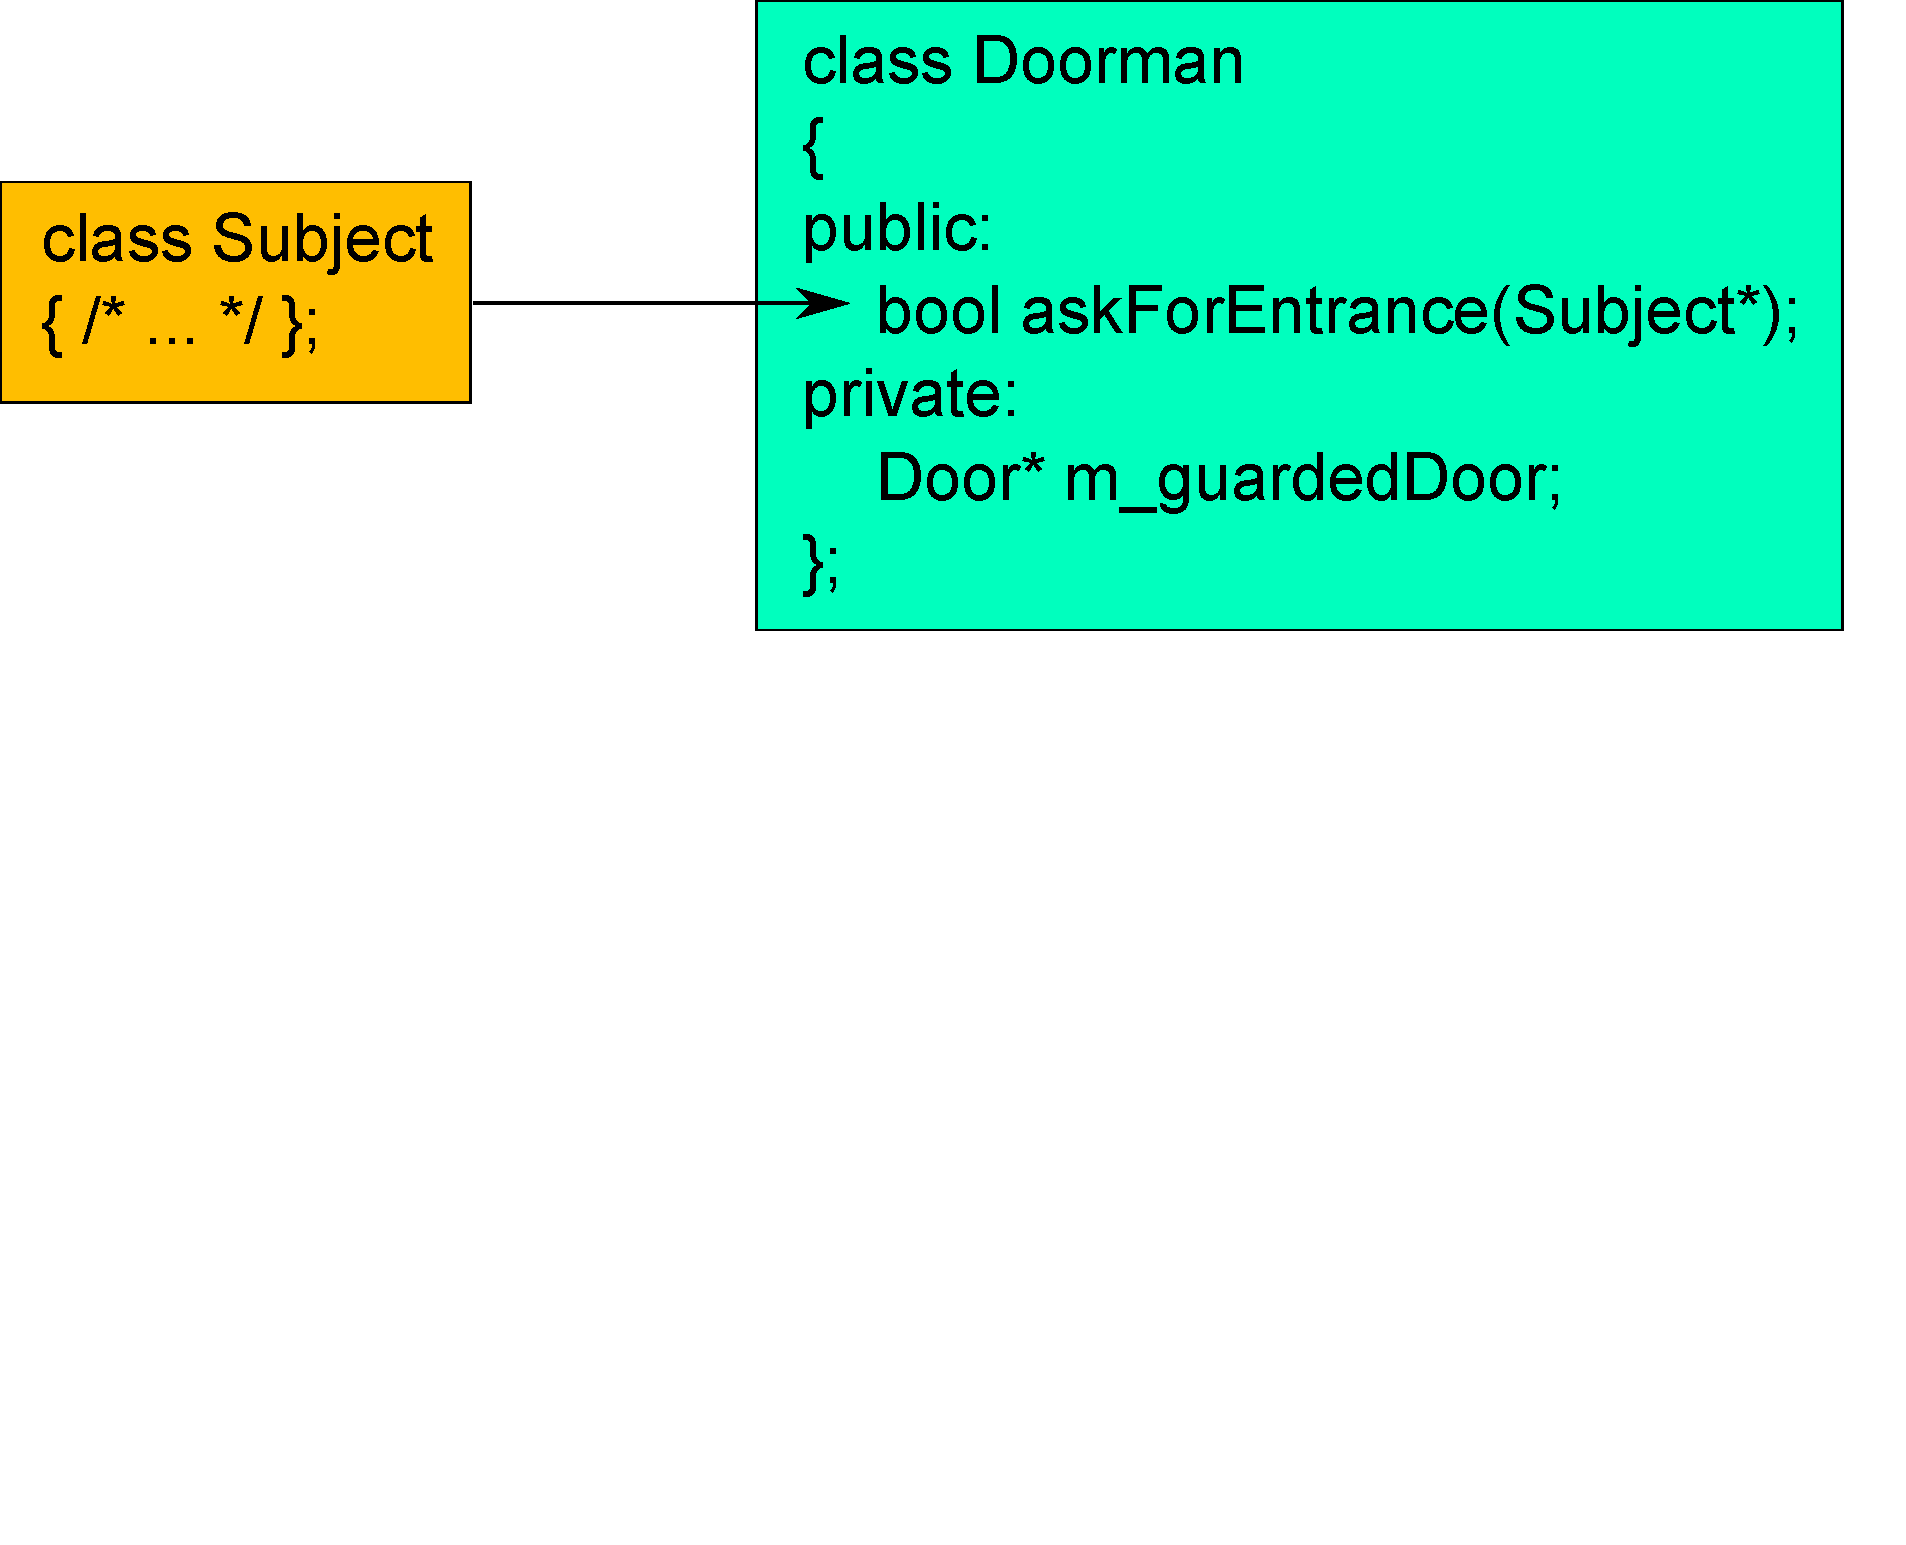
\includegraphics[height=0.75\textheight]{images/without-friendship-0} }
	\onslide*<+> { 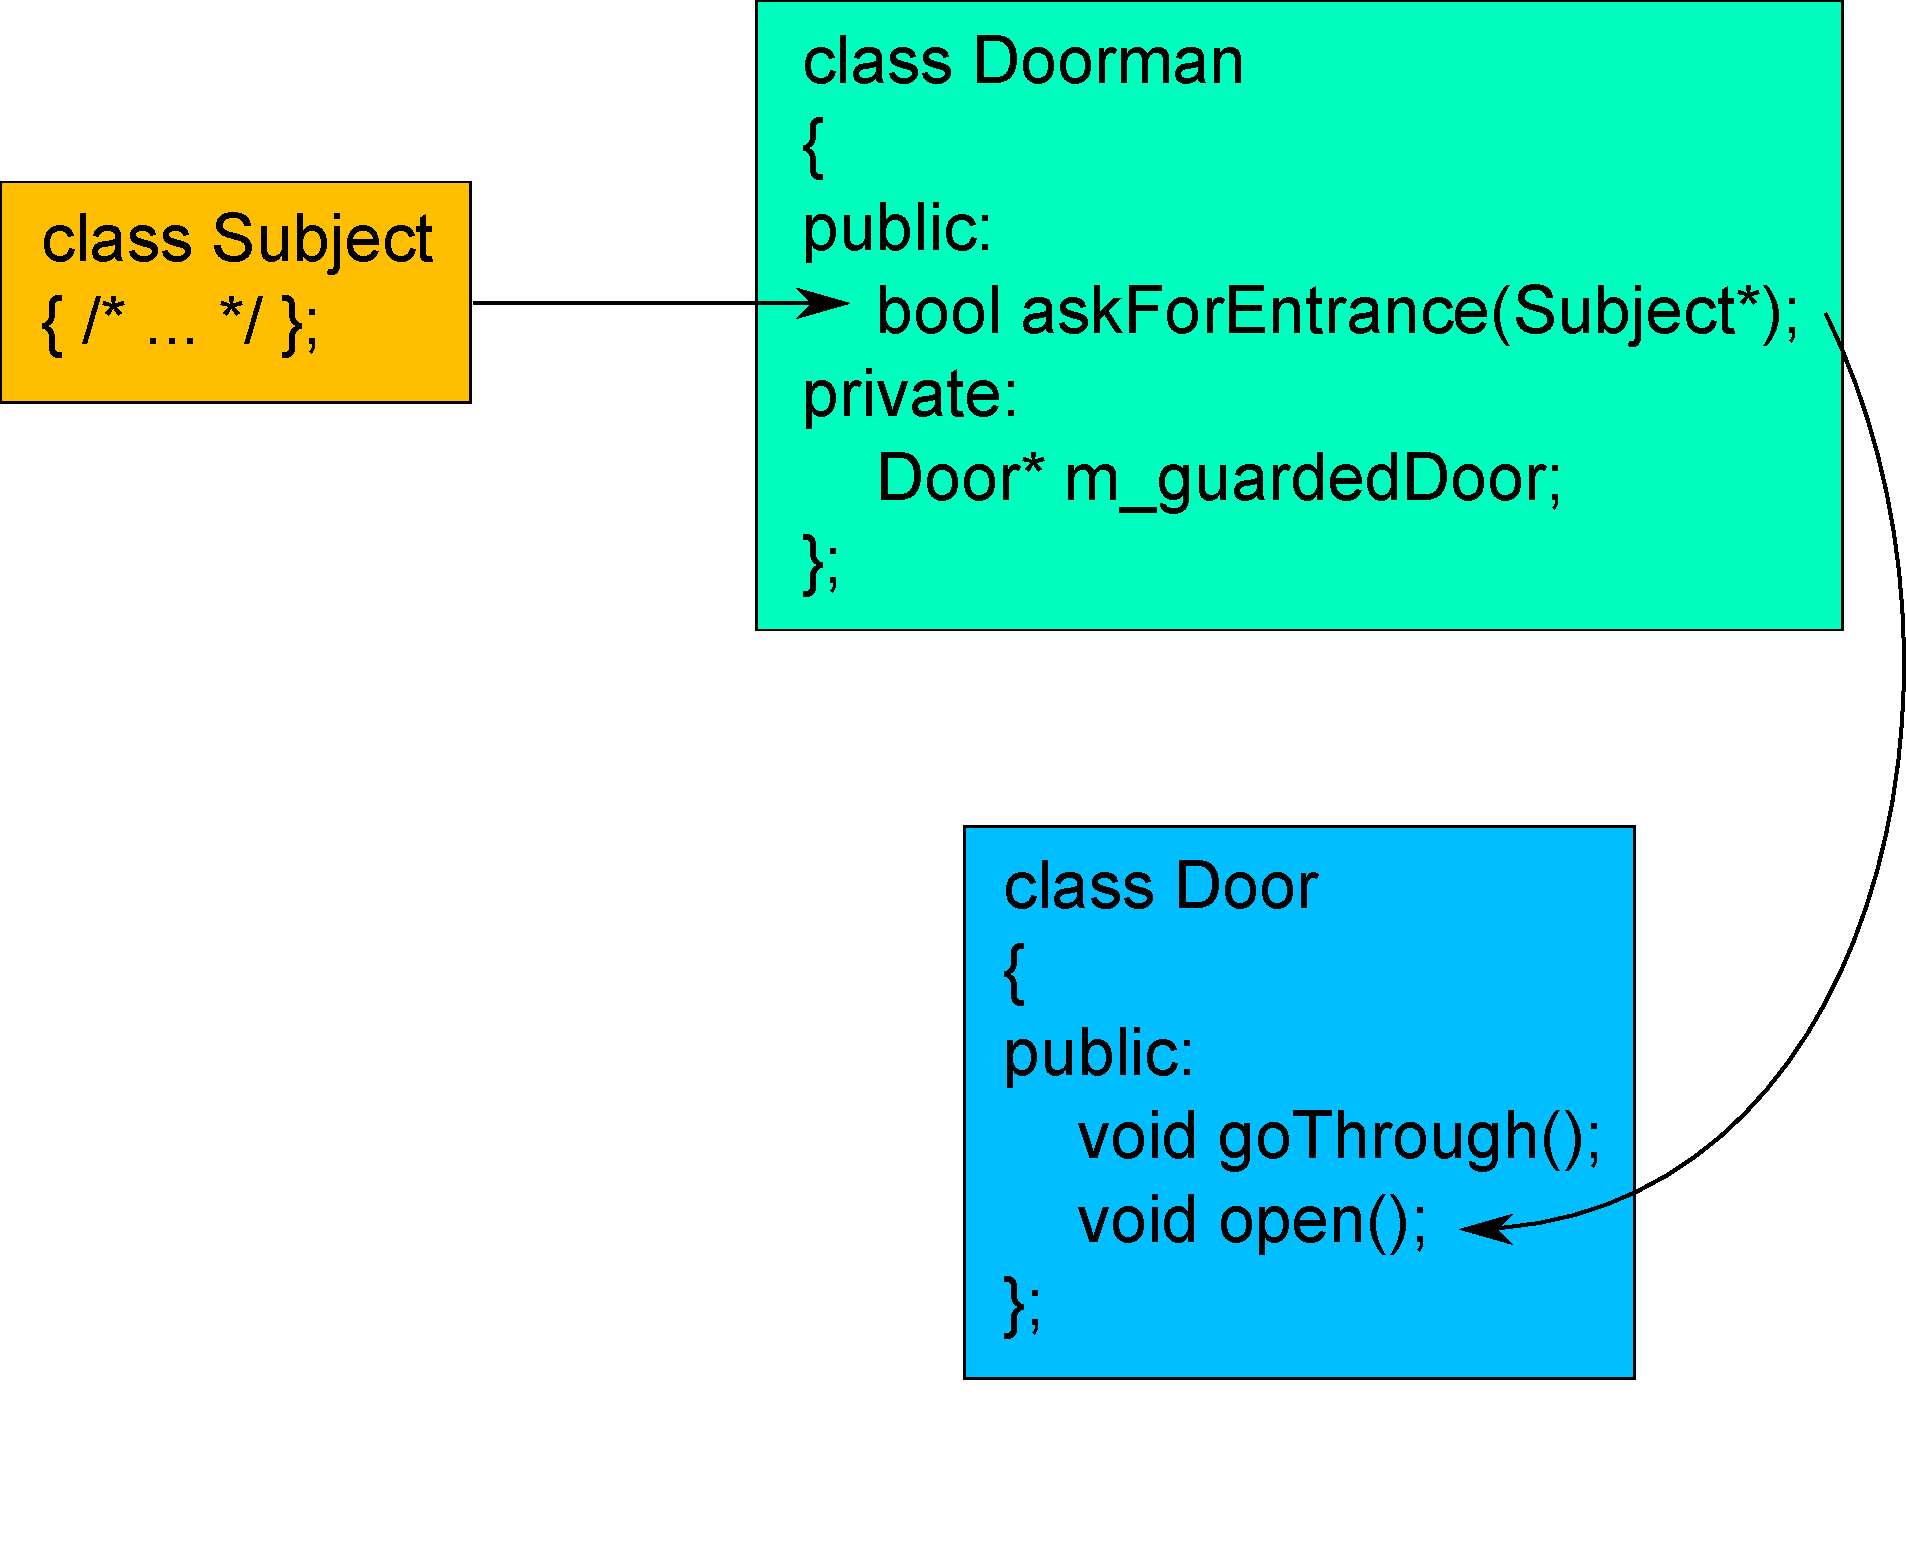
\includegraphics[height=0.75\textheight]{images/without-friendship-1} }
	\onslide*<+> { 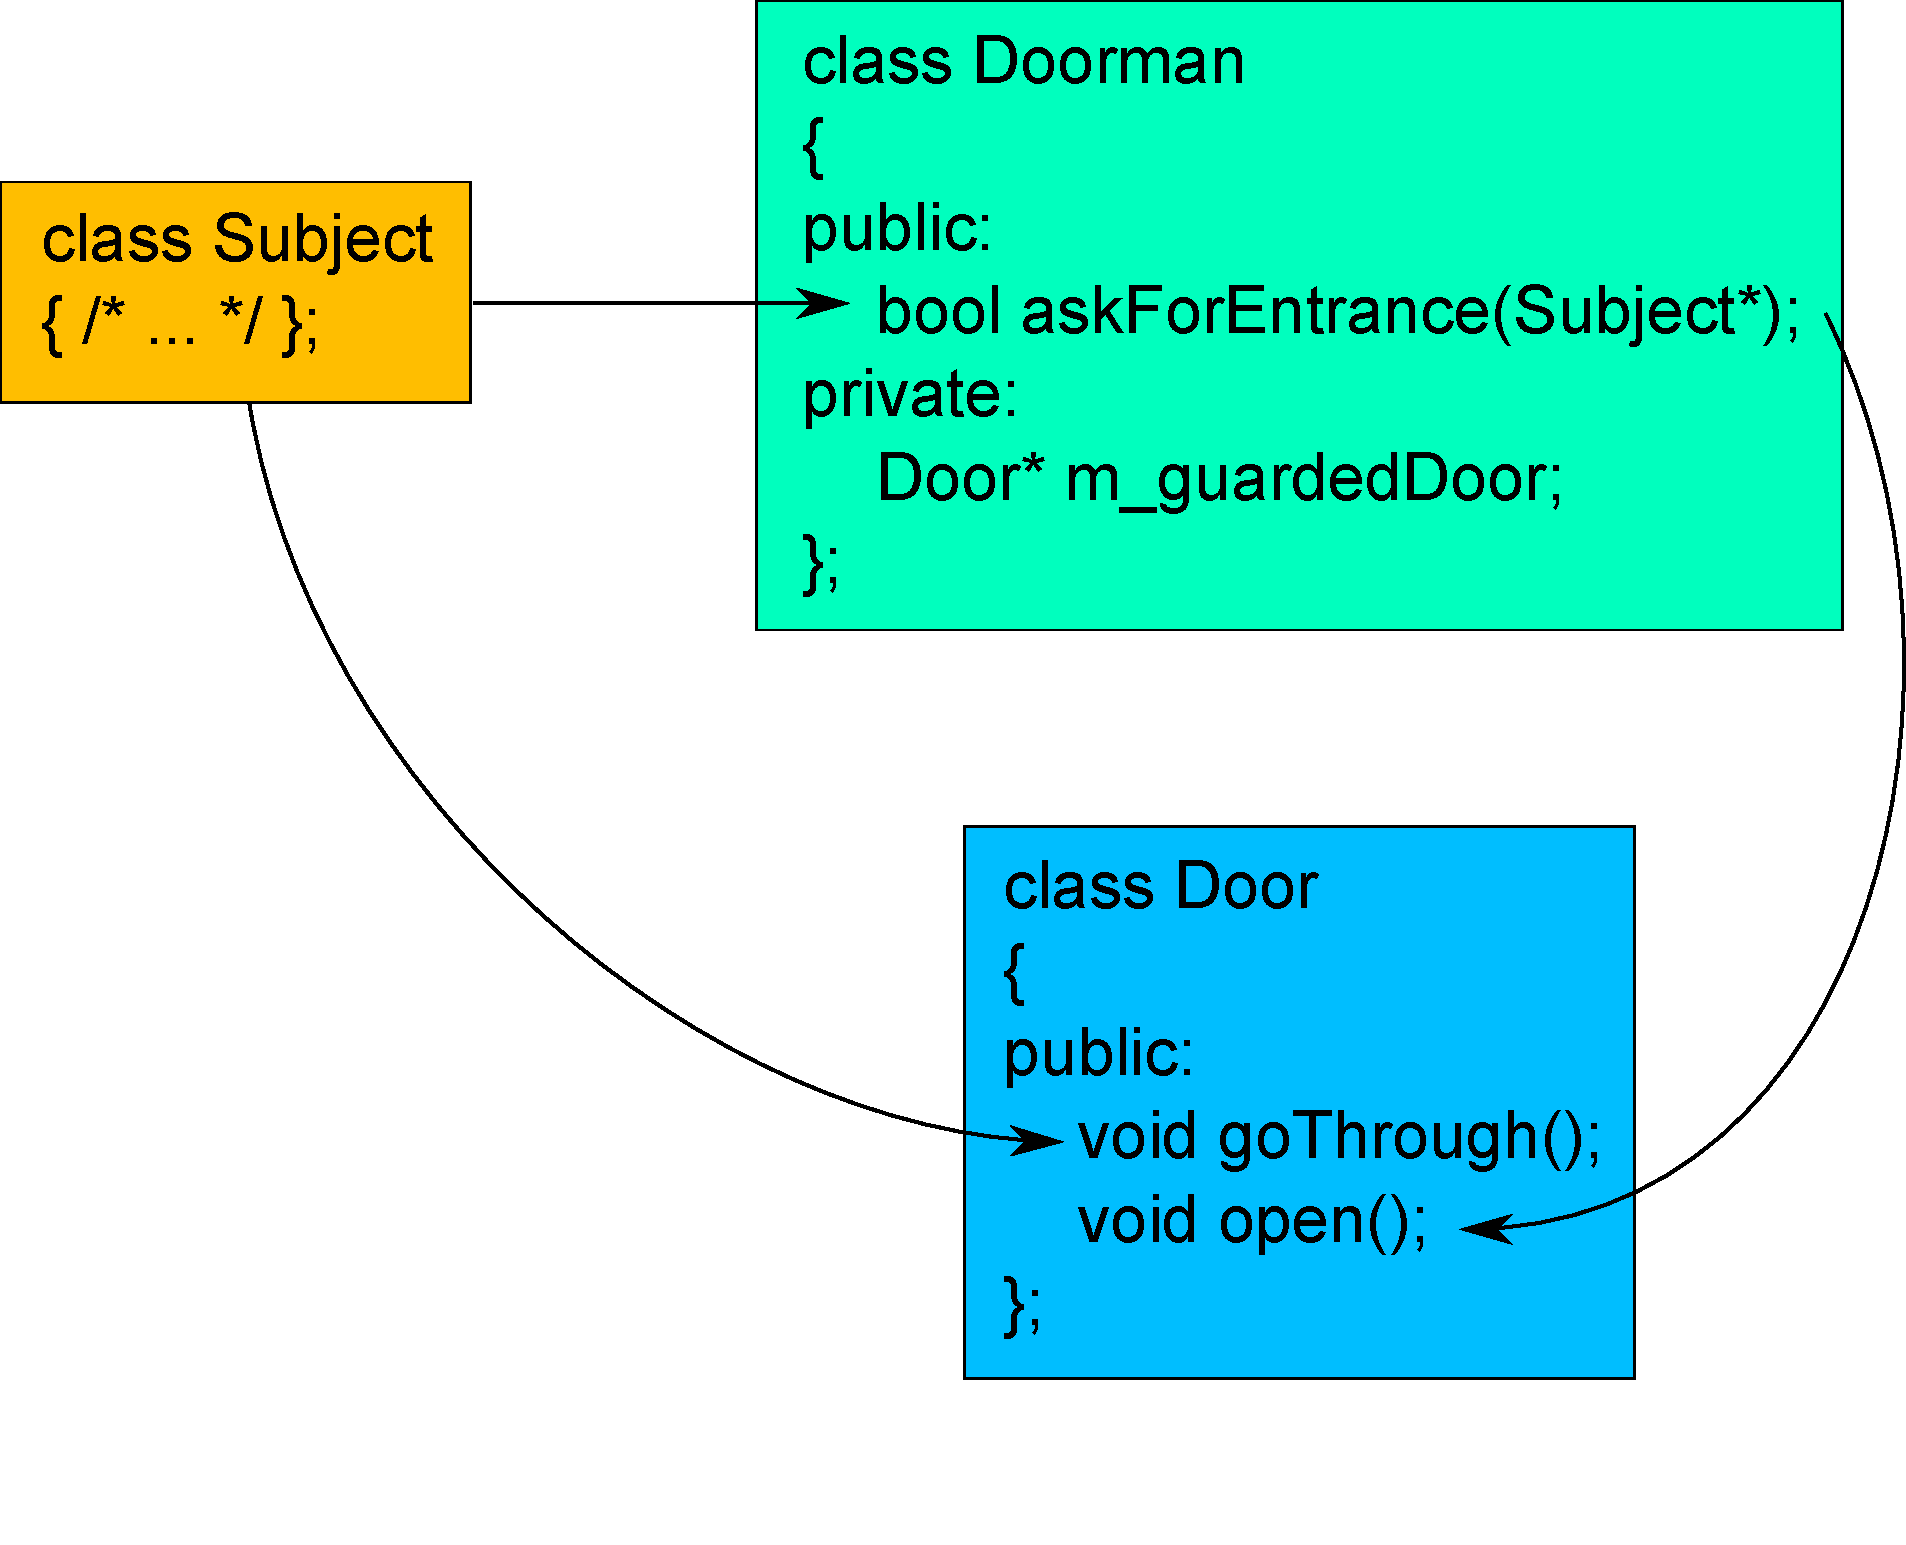
\includegraphics[height=0.75\textheight]{images/without-friendship} }
	\onslide*<+> { 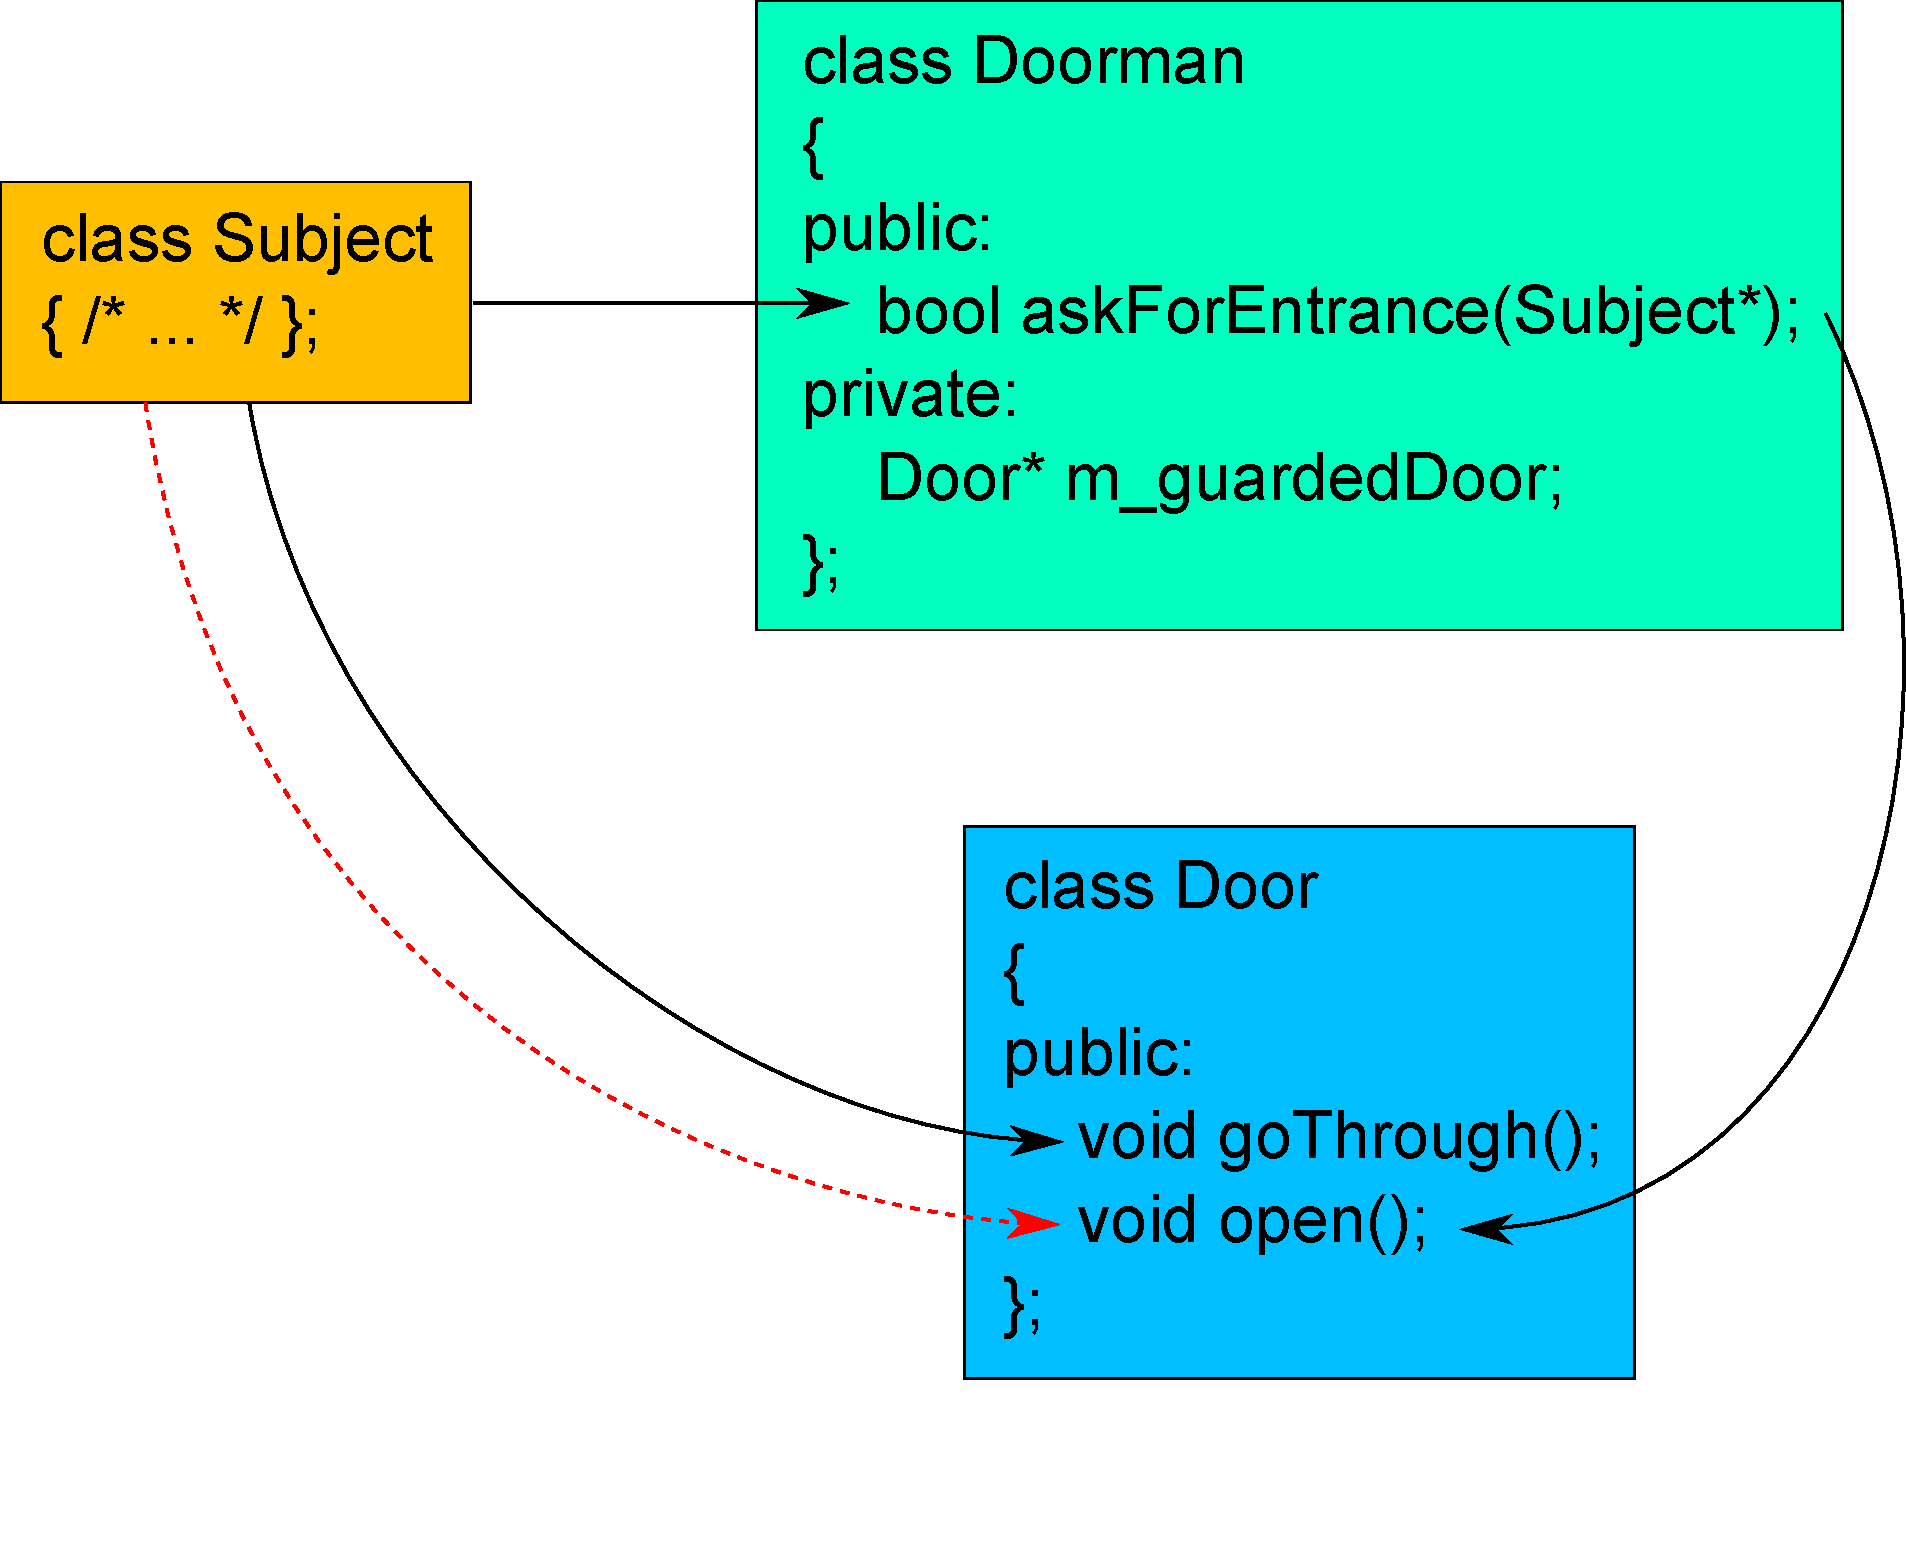
\includegraphics[height=0.75\textheight]{images/without-friendship-unauth} }
	\onslide*<+> { 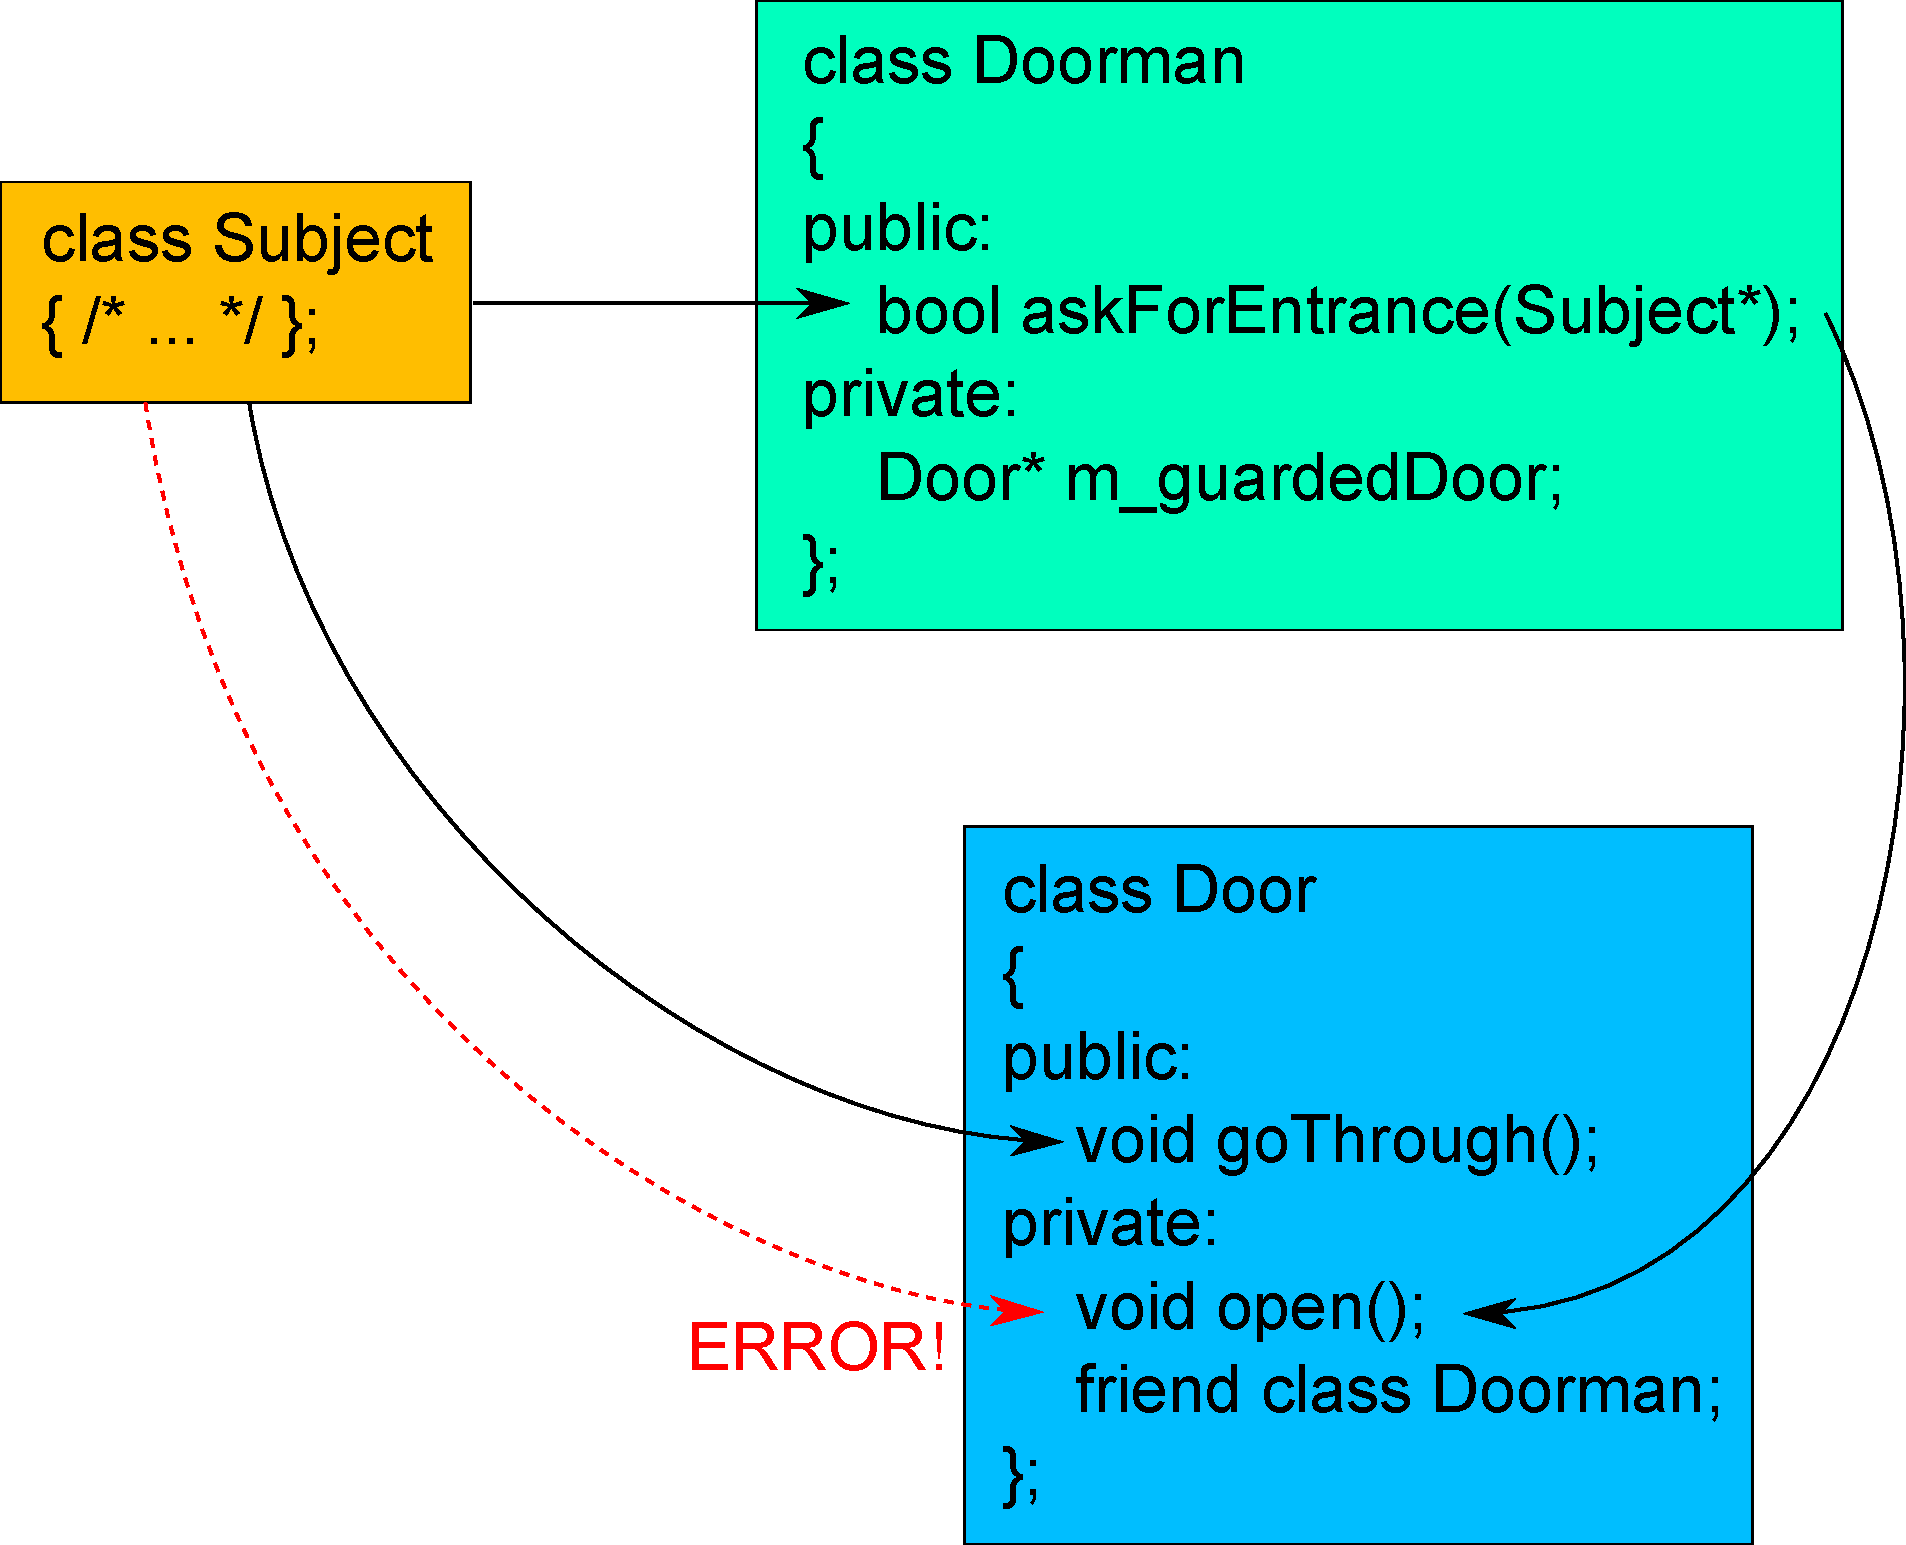
\includegraphics[height=0.75\textheight]{images/with-friendship} }
\end{frame}





\subsection{friend}

\begin{frame}[fragile]{Syntax}
	\begin{lstlisting}
struct B;
void globalFunc(B b);
struct A { void foo(B b); };

struct B {
    // public, private, protected or nothing at all
    friend class A;
    friend void globalFunc();
private:
    int m;
    void doInternal();
};
	\end{lstlisting}
	
	\pause
	
	\begin{block}{Syntax (Standard, 11.4)}
		Friendship gewährt man durch eine Deklaration in der Klassen-\emph{member-specification} mit \emph{friend-specifier} und für einen Typen mit \emph{elaborated-type-specifier} (7.1.5.3).
	\end{block}
\end{frame}


\begin{frame}[fragile]{Wirkung}
	Siehe Standard, 11.4.
	Hauptsächlich: man darf in member functions der befreundeten Klasse auf private und protected member der Freundschaft-gewährenden Klasse zugreifen.
	
	\begin{block}{Beispiel}
		\begin{columns}[t]
			\column{0.55\textwidth}
			\begin{lstlisting}
struct B {
    friend class A;
    friend void globalFunc();
private:
    int m;
    void doInternal();
};
			\end{lstlisting}
			
			\column{0.45\textwidth}
			\begin{lstlisting}
void globalFunc(B b)
{
    b.doInternal();
}
void A::foo(B b)
{
    b.m = 42;
    b.doInternal();
}
			\end{lstlisting}
		\end{columns}
	\end{block}
\end{frame}


\begin{frame}{Hinweise}
	\begin{itemize}
		\item Friendship wird nicht vererbt!
		\item Friendship ist nicht transitiv!
	\end{itemize}
\end{frame}
